% Sammenligning:
% 	- Sammenligning om implementasjon OG kjøring om: Bra/dårlig ved:
% 		- kjøring av de to
% 		- implementasjon av de to
% 		- sensor(best for KANN)
% 		- kjøretid (effektivitet for ulike 'scenarios')
% 		- over nettverk : best for KANN.
%


%todo : analyser avviket fra KN til SN sine depolrarisasjonskurver. Kvifor finnes dette avviket? Kva er greia? Lag mikroplott for stigende og synkende flanke. osv.

\chapter{Comparison and result} 




Skrive innledning: Kva er felles for de to implementasjonane: Kva er kjendt i biologien, og kva er utelatt for desse implementasjonene?

Kva har dette til felles med andre implementasjoner, og kva er gjort bedre i denne impelementasjonen i forhold til andre varianter av ANN (1. gen., 2. gen. og 3.gen. ANN).

\section{Forskjell i implementasjon}
Skrive at forskjellen mellom gamle og nye varianten av 3.gen. ANN (SANN) har mykje til felles med forskjellane mellom Moore vs. Mealy Auromata.

Den gamle varianten er for så vidt den som er mest intuitiv å implementere / designe. Denne ser på umiddelbar tilstand (depol. verdi) for nodene. Dersom denne depol. kommer over terskel vil noden gi output til alle sine utnoder.
Dette er en direkte simulering av det biologiske neuronet. Kan beskrives (direkte?) med Moore Automata.

For den foreslåtte varianten vil Mealy automata beskrive systemet bedre. Her er det 'state' for noden og i tillegg input som gir ut-oppførselen.
[skriv kva "utoppførsel" betyr. Alltid samme output (før synapsen) for den Moore-Automata varianten av SANN. For Mealy variant vil output være en flyttallsvariabel]
[skriv kvifor denne tanken kom -- at enkel kraftig prosessor vil være oppmot like effektiv med større flyttalsoperasjoner som ved enkle boolske transmissjoner (tjaneei..)
Dersom vi har mulighet er ferre større operasjoner bedre for den serielle CPU enn mange små operasjoner.]

[Skriv at implementasjonen viste seg å bli meir omfattende enn først tenkt. Skriv om pEstimatedTaskTime og anna ekstra tidsplanlegging]




\section{Testoppsett for sammenligning av KANN og SANN}
Skrive at design av/teorien bak  de to impelmentasjonene er så forsjellig at det er vanskelig å sammenligne de to. En enkel kjøring vil ha statisk input (ikkje-endrende input).
Mealy varianten av SANN (KANN) er spesialisert for ANN med dynamisk (endrende) input. Vil gi eit vanskeligere testoppsett for sammenligning av de to. Lett å implementere for KANN, vanskeligere å implementere for SANN.
(Da må eg ha egene sensor-neuron som er spesiallaga for å sense en slik dynamisk state).

	\subsection{Fleire testoppsett? Beskriv de ulike oppsetta, og kvifor!}
	\subsection{Teste for oppdelte nett: med koblinger med lite overføring/endring i overføring}

\section{Skrive kva som er utelatt} % Kanskje heller i discussion?
Kva var originalt planlagt, men viste seg å bli for mykje arbeid?

\begin{itemize}
 	\item Synaptisk plastisitet.
\end{itemize}




\subsection{Comparison between the transient time course of the depolarization of the K auron and s auron ,   Vettafaen kor det skal ligge}
To compare %the implementation of (?)
			the two models, we will start with comparing the depolarization of a single node from each model.
The same input to the two nodes should optimally give the same transient time course of the depolarization.

Because of the complexity of each node in a neural network, we cannot use a network of neurons to generate an equal input to the analyzed neuron. 
At least not before we now that they give the same output.
My solution for this is 
%The solution for this was
						to devise an own underclass K\_sensor\_auron for the $\kappa$ANN model and s\_sensor\_auron for the SANN model, that gives an output based on some ``sensor function''.
This sensor function can be made to give an output appropriate for comparing the variants of the node.

Both sensor classes are constructed by sending a function pointer into the constructor of the object. 

\begin{lstlisting}
K_sensor_auron::K_sensor_auron(
  std::string sNavn_Arg, double (*pFunk_arg)(void) ) 
     :  K_auron(sNavn_Arg)
{
	// Assign the sensor function:
	pSensorFunction = pFunk_arg;
	// Add to pAllSensorAurons list:
	pAllSensorAurons.push_back(this);

	...
}
\end{lstlisting}

Where the member variable \emph{double \mbox{(*pSensorFunction)(void);}} is a function pointer that is assigned the the function pointer adress that is sent in as an argument in the class constructor.
%This causes \emph{pSensorFunction} for point to the function sent in as an argument in the constructor.'
The variable pAllSensorAurons is a list containing all the valid sensor objects, used for updating the value of each sensor neuron when \emph{time\_class::doTask()} iterates time. %i time_class::doTask()

\begin{figure}[hbtp!]
	\label{figComparisonBetweenSsensorAndKsensorDepolCurve}
	\centering
	%\begin{center}
		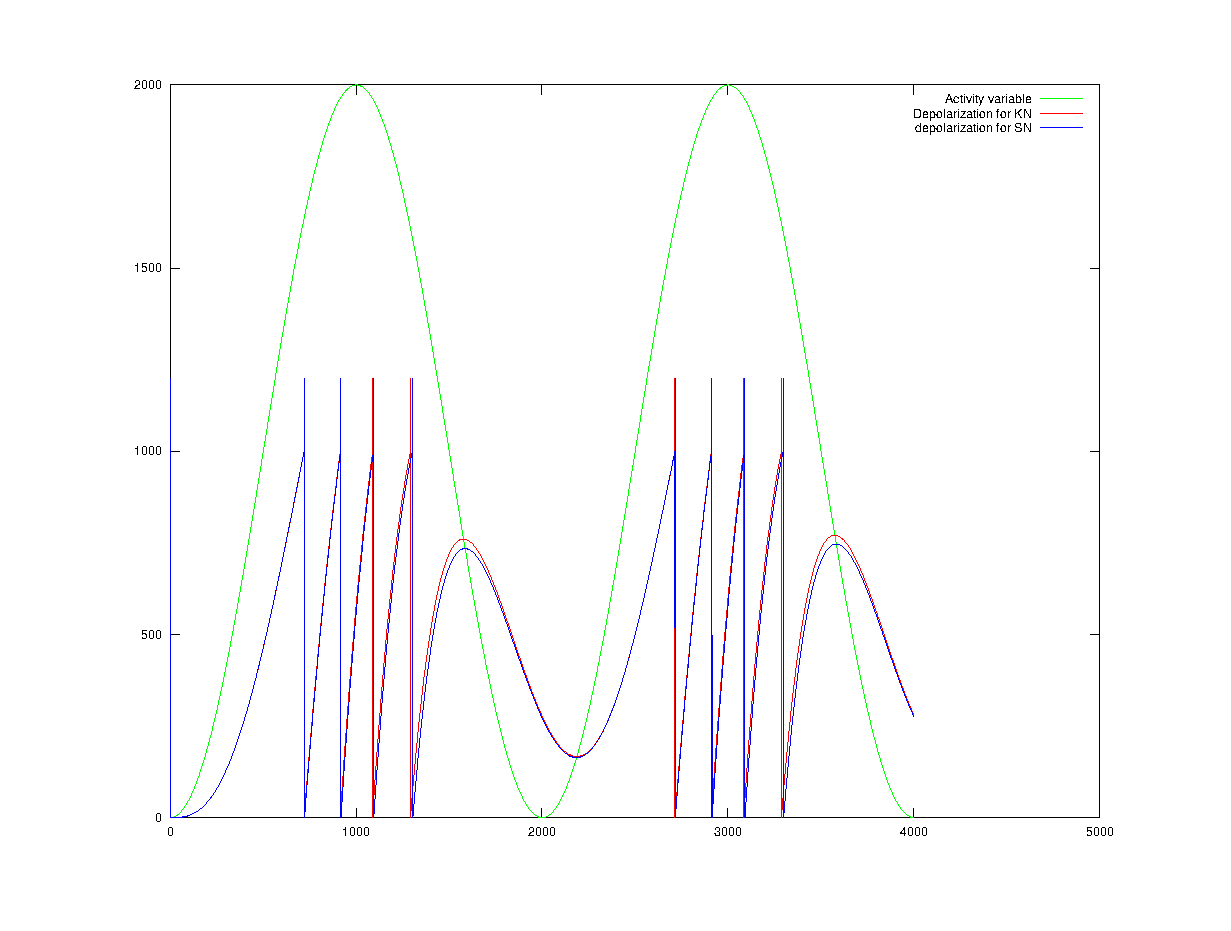
\includegraphics[width=0.95\textwidth]{eps_Comparison_between_the_two_sensors__depol.eps}
	%\end{center}
	\caption{The depolarization curve for a SANN node and a $\kappa$ANN node with the same input. The sensor function is also plotted for analysis of the result.}
\end{figure}

%The sensor function used for the comparison of the time course of the depolarization of a single node is 
The sensor function used has the formula $f(t) = \tau (1 + cos( \frac{\pi \, t}{1000} ))$, where $\tau$ is the firing threshold for the neuron. 
For the K\_auron the activity variable is at each time step set to this variable. 
When K\_sensor\_auron changes its activation level, we do this by sending the sensed signal to the dendrite. 
This is very simular to the way it is done in biology. %Evt kan eg skrive at "this is strongly inspired by nature".
%referer.
%Beste for refereringa over er nok å skrive om dette i BiologiskeSystemer.tex, og referere til plassen det står. 

This implementation is strongly inspired by the biological neural system, and the stimuli is sent to the dendrite as any synaptic input.
For the K\_sensor\_auron this gives the code
\begin{lstlisting}
  changeKappa( dSensedValue - dLastSensedValue ); 
\end{lstlisting} %Eller så kan vi gjøre det direkte. (sette Kappa til målt verdi. har impa begge..)
and for the s\_auron we have
\begin{lstlisting}
  pInputDendrite->newInputSignal( (*pSensorFunction)() * ALPHA ); 
\end{lstlisting} % TODO Forstå greia med ALPHA!


Because of the mechanisms implemented for synaptic transmission in $\kappa$ANN is based on the derived, we change $\kappa$ by the discrete variant of the derived; 
The current value minus the last value or dSensedValue - dLastSensedValue.
For the s\_auron we incoorporate the time constant T as $\frac{1}{T} = $ ALPHA by sending the above listed input to the s\_sensor\_auron's dendrite.


In figure \ref{figComparisonBetweenSsensorAndKsensorDepolCurve} we can se the results. 
As can be seen, the depolarization of the K\_auron and the s\_auron is quite simular.
There is a small difference between the curves.
%It is hard to know the specific reason for the error in this implementation.  In the following section I will discuss possible explanations.

What is interesting about this curve is that it seems that the depolarization curves follow eachother exactly %Dette er rett stavemåte: exactly (google translate)
for the rising phase of the sensor curve. For the falling phase of the curve we get some difference between the depolarization of the SN and the $\kappa$N.

%After a more thorough analysis of the error, it seems that the difference is an effect based on the concept of a truncation error. %Sjekk wiki. Dette er engelsk ord for integralfeil.
For discrete integration we may get something called the trunctation error. The ``local truncation error'' is the immediate error after each time step. 
The ``global truncation error'' is the error following integration many local truncation errors. 
The global truncation error is defined as the absolute difference between the approximated solution and the actual solution. 

\subsubsection{Trunctation error of the SN} %Kanskje skrive "Spiking Node". Hugs at overskrifta blir også oppført i "index".
In SANN each node is modelled as a leaky-integrate-and-fire neuron.
When the depolarization of the SN is updated, the leak of the neuron calculated as the previous value times the leak constant.
\begin{equation} %TODO Introduser denne ligninga tidligare i oppgava. Her skal eg bare skrive siste del av den:    v_t = (1-\alpha) * v_{t-1}  
	v_t = v_{t-1} - v_{t-1} * \alpha = (1-\alpha) * v_{t-1}  
\end{equation}
The discretization of the system introduces a small error, the local truncation error, that varies with the size of the time step and the derived of the value function $\dot{v}(t)$. %"local truncation error"

The leak is calculated as the $-\alpha v_{t-1}$.
When $\dot{v}(t)$ is positive, $v_{t-1}$ is less than the value $v_t$, varying with the size of the time step and the differentiated value function $\dot{v}(t)$.
When $\dot{v}(t)$ is negative, we get the oposite result.

Each small error is integrated up to a larger error, the global trunction error. 
If some situation is analyzed where the value is the same as the initial value, the integral of the derived over this interval is per definition zero.
Global trunctation error will then dissapear. 
This further implies that for a continous signal that varies around some working point, the global trunctation error will not diverge.  %google sa at det heite "diverge"

The depolarization of a neuron have a discontinuity when the neuron fires an action potential. 
When the neurons depolarization reaches the firing threshold the value is reset to $v_0 = 0$.
In other words, each time the value of a node reaches a positive threshold, the value is reset.
In this case the global trunctation error will continue to grow, and the difference between the value curves for the SN and the $\kappa$N becomes %TODO Ikkje dette. Skriv heller eit utfall som Stavdahl vil syns er SKUMMELT!

To se if this is the backgound for the error, we isolate the error by giving the sensor aurons a constant sensor function, with an action level of $\kappa = 1.5 \tau$.
\begin{figure}[hbtp!]
	\label{figComparisonBetweenSsensorAndKsensorDepolCurveCONStActivityLevel}
	\centering
	%\begin{center}
		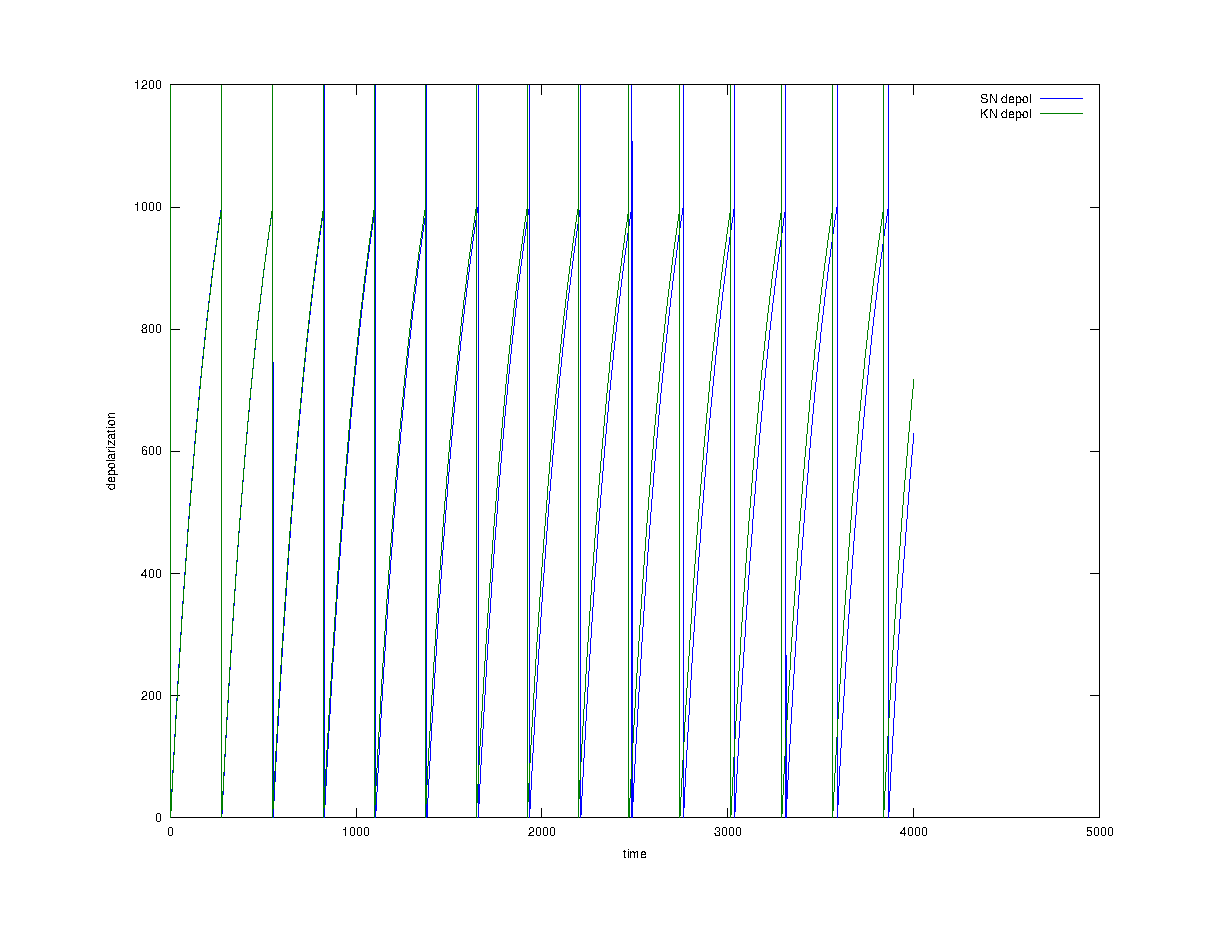
\includegraphics[width=0.95\textwidth]{eps_comparison_between_KN_and_SN_ConstKappa.eps}
	%\end{center}
	\caption{The depolarization curve for a SANN node and a $\kappa$ANN node with the same input. The sensor function has an input equivalent to an activation level of $\kappa = 1.5 \tau$.}
\end{figure}

The result is presented in fig. \ref{figComparisonBetweenSsensorAndKsensorDepolCurveCONStActivityLevel}.% .eps
If the previous analysis of the problem is sound, the SN should have a depolarization that is higher than is should be.
This implies than the depolarization curve for the SN should be ``before'' that of the $\kappa$N, which is the opposite of the situation of fig. \ref{figComparisonBetweenSsensorAndKsensorDepolCurveCONStActivityLevel}.

\subsubsection{Rounding errors}
After a more thorough analysis of the error, it seems that the difference is an effect of a rounding error.

If we change wievpoint on the error and see the difference between the two cuves as an effect of time, we can say that the $\kappa$N's depolarization curve lies before the SN's depolarization curve.
This implies that the $\kappa$N fires before the SN, and thus starts earlier on the depolarization for the next period.

In many programming languages a float is always ``rounded down''. This means that the %Det som står etter komma
is removed from the number, and the integer becomes the same as the integer part of the number.

When the $\kappa$N calculates the estimated firing time, this calculation is done in a double precision floating point number. 
To use this in the scheduler is must first be transformed to an integer variable. When this time step arrives, the task is executed.

\begin{figure}[hbtp!]
	\label{figComparisonBetweenSsensorAndKsensorDepolCurveFIXEdError}
	\centering
		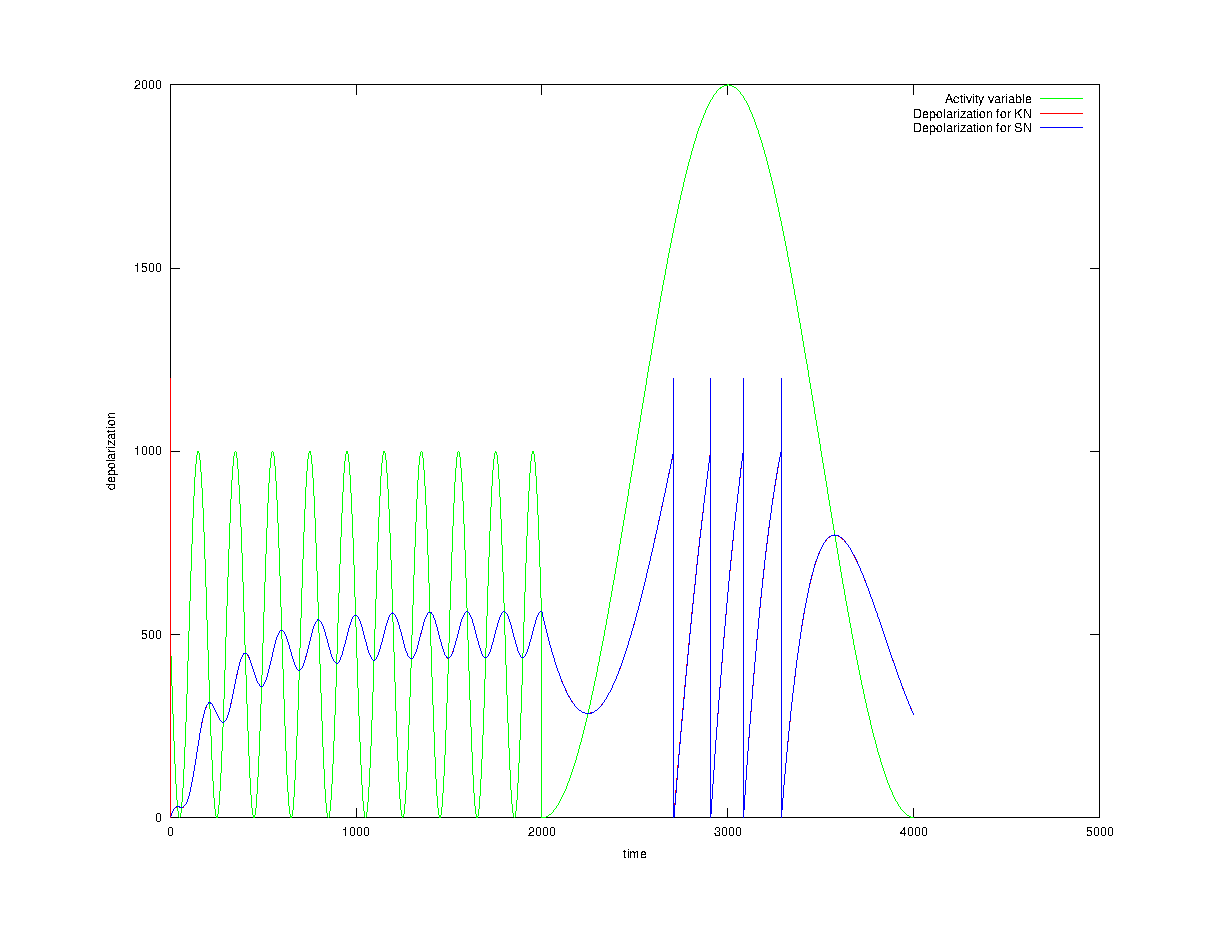
\includegraphics[width=0.95\textwidth]{eps_Comparison_between_the_two_sensors__depol_FIKSA.eps}
	\caption{Comparison between the SN's and $\kappa$N's depolarization curve. The sensor function is also plotted.}
\end{figure}

If we instead round to the closest integer, by adding $0.5$ to the float before it is converted into an integer, we get the depolarization curve presented in fig. \ref{figComparisonBetweenSsensorAndKsensorDepolCurveFIXEdError}.
In the improved depolarization curves for the auron, the error is small and can not be seen on the plot.

%Ikkje heilt sikker på om det er heilt rett: størst etter "rising flank of the ..", Bli heilt sikker på dette.
The error is largest after right after the rising flank of the activity variable's curve, the value of the sensor function.
For the situation in fig. \ref{figComparisonBetweenSsensorAndKsensorDepolCurveFIXEdError} this is at time t=3000.
At this time iteration the value of the SN is 1.015 more than the value of the $\kappa$N. 

This deviation is substantially smaller that the deviation that came from the rounding error, and it shows that the analysis made in the previous subsection is correct. %gjør om: ikkje "correct" men kanskje mindre påståelig?



% TODO KANSKJE :   \subsection{Floating point calculation pitfalls}
%                  Skriv om mulighetene for feil når man bruker float/double.


% - integralfeil for SN
% - Integralfeilen kommer antagelig av at lekkasjen  
% - For SN vil lekkasjen regnes ut fra verdien ved forrige tissteg. Denne diskretiseringseffekten vil forplante seg i at for positiv derivert av depol-kurva vil SN-depol være litt over, og for negativ flanke : motsatt.
% 		Dette er fordi lekkasjen regnes ut fra forrige verdi, som for stigende flanke er mindre enn den noværande verdien, og vi får en mindre lekkasje => for stor verdi.
% - denne feilen vil nulles ut for eit periodisk signal uten sprang (over en periode vil integralet av positiv flanke og neg. flanke bli null.
% - dersom vi har eit sprang, eller enda verre: eit sprang som alltid ligger etter en viss mengde med pos. flanke, vil vi få summert opp integral-feilen.
% For auronet vil depol settes lik 0 etter en viss mendge pos. flanke for depol. kurva. Dette skaper problemet.

% Eg har også vurdert om det er feil fra implemenasjonen: at de har ulik refraction time, MEN eg trur ikkje dette: 
% 		En slik feil ville vore mindre (eit-to tidssteg per fyring) => ikkje synlig på eit plott over fleire tusen iter's.


% MEN PROBLEMET ER FEIL VEI! JEje. Drit i det!



\newpage
For the K\_sensor\_auron 

% Den lille forskjellen mellom s_sensor_auron og K_sensor_auron er noko eg kan skrive mykje om i 'discussion'.
% Eg har tanker om at det er pga. at eg bruker integer (tid) i ligningene, og vi får dermed avrundingsfeil. Litt overraska over at feilen er så liten..
% 	Det er også mulig at den lille forskjellen kommer av forskellane i korleis sensor-funksjonen blir oversatt til depol.
% 		- K_sensor_auron oversetter sensorFunk direkte til aktivitetsVariabel Kappa, mens
% 		- s_sensor_auron sender gir eit enkelt input per tidsiterasjon gitt av ligninga (W_ij / [time constant]), eller  ALPHA * W_ij
%   XXX Dette trenger grundigare analyser!


To compare the transient time course of the value of single neurons, we give them the same input and compare the deloparization plot of the two nodes.
%we need to have the same input to both nodes.
This means that we cannot use a network of nodes, as equal output of such a network demands that each node behaves eqactly the same way for the same input, give the same input to the analyzed node.




Because a network of connected neurons have a large degree of complexity, it is best to start with comparing the depolarization of single nodes.
For this I will 
For comparison of the two models, we will first compare the depolarization of a single neuron of each model.
%Because a system comprised of a network of neurons have 

The argument behind this choice is that the 


\section{Resultat for effektivitetssammenligning}





\section{Discussion}

%En eller anna plass: (ikkje akkurat her) Skriver her fordi eg har inspirasjon no, og ikkje vil leite..) 	Ja! Kanskje i "conclutions"XXX
Implementing the mechanisms of a neural simulator is not trivial, even without optimizing it for run time efficiency.
Even if this is not an important aspect of this project I have tried to, wherever possible, optimize the implementation for efficiency.
%Skrive kvifor: Om at designet er optimalisert både for generalitet (for å gjøre utvidelser/endring lettere) og for effektivitet. DETTE for å kunne bruke implementationen videre (personlig, eller for andre).

The functions that are most often called are inlined. This means that I have given a hint to the compiler to put the compiled code wherever the functions are called.
This causes the function calls to run faster but also increases the size of the executable file, so this should be used with caution. %Kanskje skrive dette, men også da skrive størrelse på endelig program. ca. 0.5 M (?)
For this implementation, size will not be a problem. %Kvifor?
Inlining of functions are still kept to a minimum, in case of further work on this software. %skriv annaleis. Kvifor "in case of further work on this software."? Forklar bedre, eller skriv om (anna argumentering).

Also in other parts of the implementation, the code is written with a focus on possible future expantion.
%Difor er ting laga enkel å forstå for en som kan nevro: oppsettet av nodene er lagt opp som det biologiske neuronet.
The object model is designed to be general for the two models, both to make the two implementations more comparable for this project and to make the implementation better suitable for future comparison.

The design of each node is based on the biological neuron to be more intuitive for programmers with knowledge of neuroscience. 
This is not only to make the implementation easier to use for potential future programmers, but also because little is known about what is important in neuroscience.
If the implementation is constructed strongly inspired by the emulated system, with multible elements constructed in the same way as the original system, expantion and modification of the indivitual elements involve less effort.
Say, for example, that new aspects are discovered tomorrow. In this case, the code can easier be modified after this discovery.

This principle does not only account for future uses by other programmers.
In multiple occations, aspects that are where new to me have been implemented at after the main functionality of the classes where designed. 
This required less work because I followed principles that was important to Bjarne Stroustrup during the creation of C++; To make the design general and open and suited for any future uses.%ELLER NOKE Siter"TheDesignAndEvolution of C++".

One element that is not implemented, is axo--somatic and axo--axonic synases. 
This is synapses where the input to the postsynaptic neuron enters at other places of the neuron than the dendrite. 
In biology, most inhibitory synases have theire input close to the soma of the postsynaptic neuron. 
This will give the inhibitory input less delay compared to the exitatory input, and might be an important aspect in neural computations.
This can be implemented easily if this is found to be important for some future use of this code.

An other important aspect that is not impelented is axo-axonic synapses, linked to short term synaptic plasticity.
%XXX An axo--axonic synapse is a synase that enters the postsynaptic neuron somewhere close to one of its output synapses.
% Gjør om rekkefølgen litt. Skriv om short-term syn.p. først, så evt. axo-axonic synapses.
Short--term synaptic plasticity is synaptic plasticity that does not have any long term effect of the neuroal network (learning), only on more immedate aspects of signal transmission.
In particular, we have the synapses that gives input near the axon terminal of the neuron (axo-axonic synapses). This will alter the depolarization at the neurons output synapses. %og auke/minke mengde Ca2+ i presyn. bit av synapsen.
This will not cause any transmission to occur, only ``prime'' the presynaptic membrane of the synapse for transmission.
When the next action potential arrives, the size of the transmission will be larger than usual (or less, depending on whether the axo--axonic synapse is exitatory or inhibitory).
Again, neither short--term synaptic plasticity or axo--axonic synapses has been implemented because this was not an aspect of this project and due to time constraints.
% Skriv heller at short--term syn.p. ikkje er implementert, så axo-axonic synapses ville ikkje auka funksjonaliteten til simulatoren.
Implementing it will involve less work due to the implementation design in this code.
% Denne setninga er for å vise at det er lett å innføre. Skriv om.

If the goal of the implementation is to simulate a neural network from biology, spatial and temporal resolution is more important than efficiency of the calculation.
%When it comes to temporal and spatial resolution, this can easily be extended.
In this implementation, spatial and temporal resolution can easity be extended.
If we want to increase the accuracy, this can be done by increasing the number of elements in each node (and making the timestep accordingly smaller).
This will also make the computational efficiency of the simulator less, and the pragmatic use of the simulator will suffer.

If we need a better accuracy, and for example double the number of serial elements in each node and halve the size of the timestep, the functioning of each element will be the same.
The temporal and spatial resolution will be increased two-fold at the expence of the computational efficiency of the simulator.

With ``spatial resolution'' i refer to the ability to separate between elements located at different positions in space.
This is important for the output, scince different output synapses are situated at different locations of the neurons axon.
This will cause different transmission delays, and might be important for the neural calculations.
% Also the axon will be have more elements, and different synapses along the axon may have differenti time delay.
This gives us the ability to make a separation between ``early synapses'' and ``late synapses'' along the axon, and gives us a better spatial resolution for the simulated neuron.

The whole reason for developing the third generation ANN, spiking artificial neural networks, was the growing focus on the timing of the different events within the neural network.
This is computational demanding, and high resolution simulations is not suited for real time pragmatic uses of ANNs. For simulations used to test hypothesis in neural science, however, accuracy is most important.
The focus on generality in this implementation will therefore make the code reusable for possible future pragmatic uses and for implementing neural simulators.

If the new model is more effective than the old model for spiking neural networks, we can not now whether this is only goes for one of these uses. 
For this reason I found it best to implement as generally as possible, for future efficiancy comparison between the two models.
%Skrive eksempel: "More specifically, if we divide the axon into smaller pieces, spatial accuracy is better."
%Skriv om forskjellane mellom KANN og SANN. Her kommer kanskje største fordelen med KANN? (Kan kanskje legge inn vilkårlig antall element, til tilsvarende størrelse på 'time step').

%slutt: En eller anna plass: ....


\section{Conclution}
% DET neste er ikkje bra å ha her!
Grunnen for å fokusere på spike time, i utgangspunktet var oppdagelsen av at synapser lærer ved positiv eller negativ vekt-endring etter overføring. 
Hvilken, og kva størrelse er avgjort av når synaptisk overføring kommer i forhold til postsyn. fyring.

Etter litt har man funnet ut at desse mekanismene bare gjelder enkelte synapser, der postsynaptiske neurotransmittor receptors er spenningsavhengig for overføring. 
Med høg depolarisering, dvs lav spenning overføres meir, og bl.a. $Ca^{2+}$ som er viktig for postsynaptisk plastisitet.
"To my knowledge" har det bare blitt funnet en slik neurotransmittor-sensor i biologien. Dette er den glutamatiske NMDA receptoren.
Glutamatisk overføring har vore veldig mykje i fokus for synaptisk overføring, og det er ikkje rart at STDP har fått så veldig høgt fokus %NEI, FAEN! må ikkje argumentere mot oppgaveteksten!


\section{Notater: Kva burde eg gjordt annaleis?}
Burde ikkje bygd de to implementasjonane så lik. (?)
Det er vanskelig å sammenligne de to. For K\_auron kunne eg ivertfall droppa dendrite og kanskje axon.
Jeje - vettafaen eg.

Burde ikkje brukt så mykje tid på pEstimatedTaskTime-lista. Kanskje eg kan argumentere for at dette kan være nyttig, men for dette prosjektet er det tidssløs.


\section{Ting som kanskje er nye}
Skriv litt om optimaliseringa gjordt i SANN. Simulert asynkron tid istedetfor oppdatering kvart tidssteg.

Kalkulering av lekkasje: Kvar gang det kommer nytt input, framfor å gjøre det kvar tidsiterasjon.

\section{Kva burde eg gjordt annerledes?}
Skriv at fokuset mitt i denne implementeringa var å sammenligne de to modellene. Dette gjorde at eg satt opp auronet på eg spesiell, og ikkje-optimal måte.
(Både for effektivitet, men også for implementasjon. Det var kanskje vanskeligere å implementere modellen på måten eg gjorde det, enn nødvendig. Kann trenger bare eit auron, med synapser ut.)
Dette burde eg gjordt annerledes, og både implementering og effektivitet ville vunnet på dette.



% XXX Skriv at resetting til v_r etter AP er ikkje instantaneous. Dette tar også litt tid. For videre arbeid vil også dette bli implementert!

% XXX Skriv at KANN er en mellomting mellom fANN og SANN. Det har muligheten til å kommunisere med begge.
% 		- fANN kan overføre aktivitetsnivået sitt direkte til KANN (Kan sette $\kappa$ = input-fra-fANN) -- Begge veier (KANN: kan få info FRA, og gi info TIL fANN).
% 		- SANN kan overføre aktivitetsnivået sitt indirekte til KANN (KN kann analysere input til $\kappa$. KN kan gi output til SN (direkte))
% Det kan være dette er eit stort bidrag for ANN-verden. Dersom det i tillegg er meir effektivt, så ...


